\section{Аналитический раздел}

\subsection{Клиент-серверная архитектура}

Клиент-серверная архитектура является фундаментальным понятием, используемым для организации взаимодействия процессов (возможно, запущенных на разных вычислительных машинах).

Сервер -- процесс, способный принимать запросы, обрабатывать их и, при наличии и необходимости, возвращать ответ. Клиент -- процесс, который отправляет запросы. Таким образом, сервер предоставляет <<услуги>>, а клиент их запрашивает, инициируя коммуникацию.

Модель клиент-серверной архитектуры представлена на рисунке~\ref{client-server}.

\begin{figure}[ht]
	\centering
	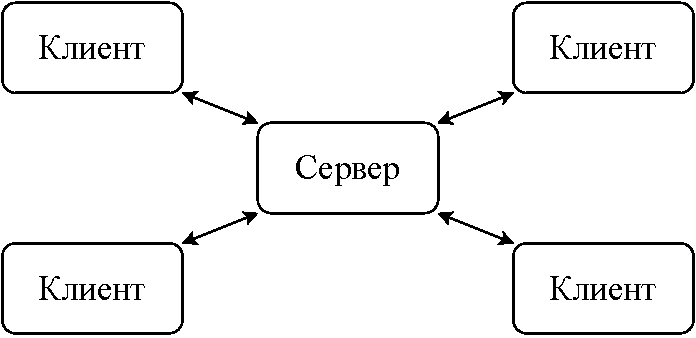
\includegraphics[scale=0.8]{img/client-server.pdf}
	\caption{Модель клиент-серверной архитектуры}
	\label{client-server}
\end{figure}

\subsection{Сокеты}

Сокет -- абстракция конечной точки соединения (взаимодействия). Они делают возможной коммуникацию процессов как на одной, так и на разных вычислительных машинах.

Подобно тому как для работы с файлами приложения используют дескрипторы файлов, для работы с сокетами они используют дескрипторы сокетов. В UNIX дескрипторы сокетов реализованы так же, как дескрипторы файлов. Разница между ними заключается в множестве допустимых операций, применимых к этим файлам.

Для коммуникации процессов по сети используется понятие порта -- конечной точки соединения, обозначаемой 16-битным целым числом. Порты используются для идентификации процесса, которому предназначается пакет. Определение процесса по номеру порта происходит в ядре операционной системы в ходе операции, называемой <<демультиплексированием>>. Это определение успешно, если некоторый процесс <<связал>> свой сокет с данным портом.

Сокет создается системным вызовом \texttt{socket()}. Его прототип представлен в листинге \ref{lst-socket}.

\captionsetup{singlelinecheck = false, justification=raggedright}
\begin{lstlisting}[caption={Прототип системного вызова socket()}, label=lst-socket]
#include <sys/socket.h>
int socket(int domain, int type, int protocol);
\end{lstlisting}
\captionsetup{singlelinecheck = false, justification=centering}

Аргумент domain определяет природу взаимодействия, включая формат адреса. Например, домен Интернета IPv4 определяется константой \texttt{AF\_INET}, а домен UNIX -- \texttt{AF\_UNIX}. Тип сокета (аргумент type) определяет его характеристики взаимодействия. Например, тип \texttt{SOCK\_DGRAM} не ориентирован на создание логического соединения, допускает отправку сообщений только фиксированной длины и не гарантирует доставку сообщений. Тип \texttt{SOCK\_STREAM} ориентирован на создание логического соединения, упорядоченность передачи данных и гарантирует их доставку. В качестве протокола (аргумент protocol), как правило, указывается 0, что означает использование протокола по умолчанию. Так, для \texttt{SOCK\_DGRAM} из домена \texttt{AF\_INET} это UDP, а для \texttt{SOCK\_STREAM} из домена \texttt{AF\_INET} -- TCP.

\subsubsection{Передача данных}

Взаимодействие с использованием сокетов осуществляется по модели клиент-сервер. Последовательность системных вызовов при использовании протокола с установлением соединения (TCP) представлена на рисунке \ref{tcp}.

\begin{figure}[ht]
	\centering
	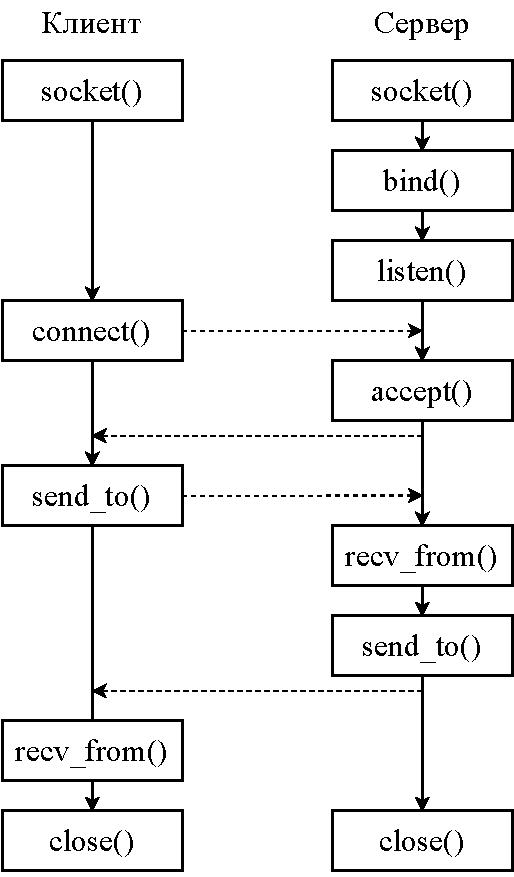
\includegraphics[scale=0.8]{img/tcp.pdf}
	\caption{Передача сообщения от клиента серверу}
	\label{tcp}
\end{figure}

Системный вызов \texttt{bind()} используется для назначения сокету локального адреса. Для сетевых сокетов определена структура \texttt{struct sockaddr\_in}, в которой явно определяется порт и IP-адрес.

Вызов \texttt{connect()} устанавливает соединение по адресу, который передается в функцию в качестве аргумента.

Когда сервер получил запрос на соединение, то будет выполнен системный вызов \texttt{accept()} -- принять этот запрос. Данный системый вызов создает копию исходного сокета и возвращает дескриптор файла нового сокета. В результате исходный сокет остается в состоянии <<listen>>, а копия -- в состоянии <<connected>>. Дублирование сокетов при принятии соединения дает возможность серверу принимать новые соединения без необходимости закрывать ранее принятые.

\subsection{Мультиплексирование}

Традиционный способ написания серверов -- использовать главный поток, заблокированный на системном вызове \texttt{accept()} в ожидании новых подключений. Как только приходит новый запрос на соединение, сервер создает новый процесс системным вызовом \texttt{fork()}. Дочерний процесс обрабатывает запрос, а родительский (главный) готов снова принимать запросы на подключение.

Чтобы избежать создания нового процесса под каждый запрос, что затратно по ресурсам, используют мультиплексирование запросов средствами API \texttt{select}, \texttt{poll}, \texttt{pselect} и \texttt{epoll}.

\subsubsection{select}

Системный вызов \texttt{select()} позволяет программе отслеживать несколько файловых дескрипторов в ожидании, пока один или несколько из них станет <<готов>> к какого-то вида операции ввода-вывода. Файловый дескриптор считается готовым, если соответствующую операцию ввода-вывода можно произвести без блокировки.

Но поскольку \texttt{select()} проектировался до появления концепции неблокирующего ввода-вывода, ряд трудностей делает его использование в современных системах нецелесообразным:

\begin{itemize}
	\item[---] Для выяснения того, какой именно дескриптор сгенерировал событие, необходимо вручную опросить их все с помощью \texttt{FD\_ISSET}, что приводит к излишним затратам ресурсов;
	
	\item[---] Максимальное количество одновременно наблюдаемых дескрипторов ограниченно константой \texttt{FD\_SETSIZE}, которая равна 1024;
	
	\item[---] Закрытие дескриптора сокета, отслеживаемого API \texttt{select()}, не в главном потоке, приводит к неопределенному поведению;
	
	\item[---] Невозможно динамически менять набор наблюдаемых событий;
	
	\item[---] Отдельно необходимо вычислять наибольший дескриптор и передавать его отдельным параметром.
\end{itemize} 

\subsubsection{pselect}

Как и \texttt{select()}, \texttt{pselect()} ждет изменения статуса нескольких файловых дескрипторов. Эти функции идентичны, за исключением трех отличий между ними:

\begin{enumerate}
	\item Функция \texttt{select} использует время ожидания, которое задано в структуре \texttt{struct timeval} (с секундами и микросекундами), тогда как \texttt{pselect} использует \texttt{struct timespec} (с секундами и наносекундами).
	
	\item Функция \texttt{select} может обновить параметр \texttt{timeout}, который показывает сколько времени прошло. Функция \texttt{pselect} не изменяет этот параметр.
	
	\item Функция \texttt{select} не имеет параметра \texttt{sigmask}, и т.о. ведет себя также как функция \texttt{pselect} вызванная с этим параметром, установленным в \texttt{NULL}.
\end{enumerate}

\subsubsection{poll}

После появления необходимости писать высоконагруженные сервера был спроектирован API \texttt{poll()}, учитывающий недостатки \texttt{select()}:

\begin{itemize}
	\item[---] Ограничение в 1024 файловых дескриптора отсутствует;
	
	\item[---] Наблюдаемые структуры лучше структурированы;	
\end{itemize}

Однако и \texttt{poll()} не лишен недостатков:

\begin{itemize}
	\item[---] Как и при использовании \texttt{select()}, невозможно определить какие именно дескрипторы сгенерировали события без полного прохода по всем наблюдаемым структурам и проверки в них поля revents;
	
	\item[---] Как и при использовании \texttt{select()}, нет возможности динамически менять наблюдаемый набор событий.
\end{itemize}

\subsubsection{epoll}

Данный API появился как логическое продолжение \texttt{select()} и \texttt{poll()}. От них он отличается тем, что позволяет добавлять, удалять и модифицировать дексрипторы и события в наблюдаемом списке.

Последовательность работы с \texttt{epoll} следующая.

\begin{enumerate}
	\item Создать дескриптор \texttt{epoll} с помощью вызова \texttt{epoll\_create};
	
	\item Инициализировать структуру \texttt{epoll\_event} нужными событиями и указателями на контексты соединений;
	
	\item Вызвать \texttt{epoll\_ctl} посредством макроса \texttt{EPOLL\_CTL\_ADD} для добавления дескриптора в список наблюдаемых;
	
	\item Вызвать \texttt{epoll\_wait()} для ожидания событий с указанием максимального числа событий, которое можно получить за раз;
	
	\item Обработать полученные события.
\end{enumerate}

Важным отличием является отсутствие необходимости просматривать весь список отслеживаемых дескрипторов.

Достоинства \texttt{epoll} следующие:
\begin{itemize}
	\item[---] Нет необходимости просматривать полный список структур в поисках той, возможно, одной, где сработало ожидаемое событие.
	
	\item[---] Есть возможность добавлять или удалять сокеты из списка в любое время. Также можно модифицировать наблюдаемые события.
	
	\item[---] Можно завести сразу несколько потоков, ожидающих события из одной и той же очереди с помощью \texttt{epoll\_wait}.
\end{itemize}

Несмотря на описанные улучшения, в некоторых ситуациях использование \texttt{epoll} нецелесообразно. Недостатки \texttt{epoll} следующие:

\begin{itemize}
	\item[---] Изменение флагов событий происходит средствами лишнего системного вызова \texttt{epoll\_ctl}, что добавляет лишнее переключение контекста;
	
	\item[---] Для каждого нового соединения необходимо вызвать \texttt{accept()} и \texttt{epoll\_ctl()} -- это два системных вызова. В случае использования poll вызов будет лишь один. При очень коротком времени жизни соединения переключения контекста могут значительно понизить производительность.
	
	\item[---] Отсутствие переносимости на платформы, отличные от Linux;
\end{itemize}

\subsection{Модели конкурентных серверов}

Самая простая модель обработки запросов к серверу -- итеративная. В данной модели сервер может может обрабатывать только одного клиента в единицу времени. Остальные клиенты блокируются до тех пор, пока не подойдет их очередь и им не будет возвращен ответ.

Для обработки нескольких запросов одновременно можно использовать следующий подход: при получении запроса на подключение для его обработки выделяется новый поток или процесс. При высокой нагрузке сервер, использующий данную модель, неэффективен, поскольку, при увеличении числа потоков или процессов, в мультизадачных системах кванты времени для обработки запросов начинают выделяться реже.

Чтобы избежать падения производительности сервера, связанного с затратами ресурсов на создания потока или процесса, используют следующие модели: pre-forking и pre-threading.

Pre-forking -- создание пула копий процесса-родителя. Запрос обрабатывается любым свободным дочерним процессом. Таким образом исключаются затраты на создание процесса под каждый запрос. При повышении нагрузки процесс-родитель может увеличить размер пула. Данная модель представлена на рисунке \ref{prefork}.

\begin{figure}[ht]
	\centering
	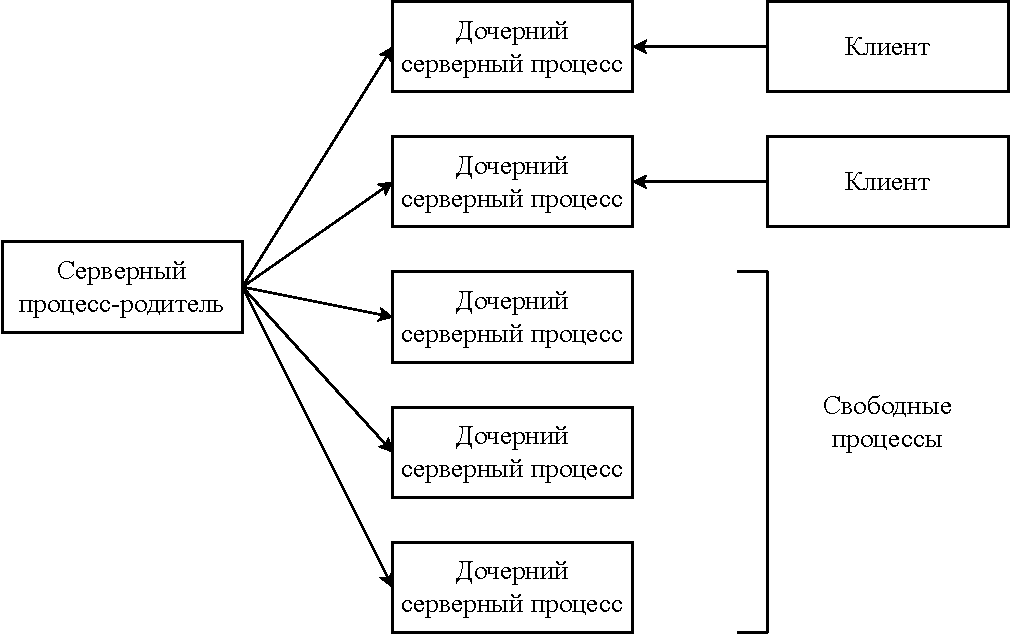
\includegraphics[scale=0.8]{img/prefork.pdf}
	\caption{Модель pre-forking}
	\label{prefork}
\end{figure}
	
Pre-threading -- создание пула потоков-обработчиков запросов. Идея данной модели аналогична pre-forking, только вместо пула процессов используется пул потоков (англ. thread pool). Данная модель представлена на рисунке \ref{prethread}.

\begin{figure}[ht]
	\centering
	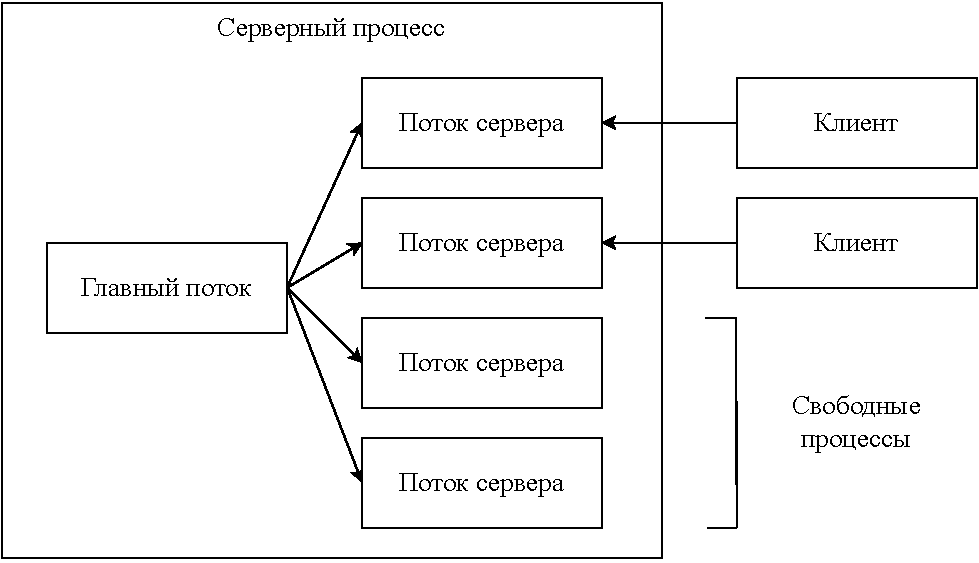
\includegraphics[scale=0.8]{img/prethread.pdf}
	\caption{Модель pre-threading}
	\label{prethread}
\end{figure}

\subsection{Проблема <<громоподобного стада>>}

Проблема <<громоподобного стада>> (англ. thundering herd problem) ставится следующим образом. Имеется M дочерних процессов (или потоков). При старте сервера все из них вызывают \texttt{accept()} и блокируются. При первом запросе на подключение все M процессов (потоков) просыпаются. Только один из них перейдет к выполнению задания на обработки, а остальные будут вынуждены снова заблокироваться.

В случае \texttt{select} с этой проблемой ничего не поделать. В случае \texttt{epoll} данную проблему попытались решить флагом \texttt{EPOLLEXCLUSIVE}, который устанавливается вызовом \texttt{epoll\_ctl}. Данный флаг устанавливает монопольный режим пробуждения для файлового дескриптора \texttt{epoll}, ассоциируемого с файловым дескриптором fd. Когда данный флаг установлен, один или несколько файловых дескрипторов \texttt{epoll} получат уведомление о событии на \texttt{epoll\_wait}. Поведение по умолчанию (без флага) -- оповещение о событии вообще всех файловых дескрипторов.


\subsection*{Вывод}

В данном разделе были проанализированы способы проектирования многопользовательских серверов. Были рассмотрены 4 модели, две из которых признаны наиболее эффективными: pre-threading и pre-forking. 

Также были рассмотрены основы сокетов и сетевого стека Linux, а также инструменты мультиплексирования: select, pselect, poll, epoll. Были приведены достоинства и недостатки каждого API, а также рассмотрена проблема <<громоподобного стада>> и метод её решения в случае epoll.

\pagebreak
